\documentclass[6008notes.tex]{subfiles}
\begin{document}
\graphicspath{ {images/graphmod/} }

\section{Graphical Models}

\subsection{Graphical Models}

To introduce graphical models, we start with three simple examples.

Note that previously we have been using random variables $X$ and $Y$, but here we will use $X_1$, $X_2$, up to $X_n$, as it will provide a clean way to write out the general case.

\textbf{Graphical Model of Two Independent Random Variables}

If $X_1$ and $X_2$ are independent random variables, then we know that $p_{X_1,X_2}(x_1,x_2)=p_{X_1}(x_1)p_{X_2}(x_2)$. Graphically, we represent this distribution as two circles. Because they are independent, we do not ``connect'' these two circles:

{\centering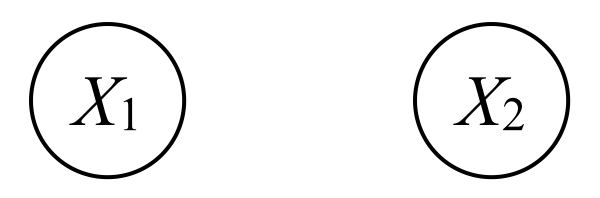
\includegraphics[scale=0.4]{images_sec-graphical-models-2-rv-indep} \par}

On a computer, we store a separate table for each of the two circles, one for $p_{X_1}$ and one for $p_{X_2}$. Later we will see that tables that we store that depend only on a single random variable need not be a marginal distribution (such as in this example). Thus, we will give the tables new names. We let $\phi_1 = p_{X_1}$ and $\phi_2 = p_{X_2}$. (Later, $\phi_i$ is the table we store that is associated with a single random variable $X_i$. In this example, $\phi_1$ and $\phi_2$ are just set to be the same as the marginal distributions $p_{X_1}$ and $p_{X_2}$.)

To summarize, the graphical model here includes the picture above (which is called a \textit{graph}) along with the tables $\phi_1$ and $\phi_2$.

\textbf{Two Possibly Dependent Random Variables}

Now suppose that we do not know whether $X_1$ and $X_2$ are independent. Then without further assumptions, we can work directly with the joint probability table $p_{X_1, X_2}$, or we can use the product rule (which importantly always holds and does not require $X_1$ and $X_2$ to be independent).

Here are three different ways we can store the distribution:

\begin{itemize}
\item (a) Store $p_{X_1, X_2}$. If we do this, then there is a single table $p_{X_1, X_2}$ that we are storing that depends on two random variables $X_1$ and $X_2$.

We introduce new notation here: a table we store that depends on exactly two random variables $X_i$ and $X_j$ will be called $\psi_{i, j}$, so in this case, we store $\psi_{i, j} = p_{X_1, X_2}$. Later, we will see examples where $\psi_{i, j}$ is not a joint probability table for two random variables.

There are no tables here that depend on exactly 1 random variable.

\item (b) Store $p_{X_1}$ and $p_{X_2 \mid X_1}$.

Here, there is one table that depends on exactly 1 random variable: $p_{X_1}$. We call this $\phi _{X_1} = p_{X_1}$.

There is one table that depends on exactly 2 random variables: $\psi _{1, 2} = p_{X_2 \mid X_1}$. (This $\psi _{1, 2}$ is different from the one in (a).)

\item (c) $p_{X_2}$ and $p_{X_1 \mid X_2}$.

Here, there is one table that depends on exactly 1 random variable: $p_{X_2}$. We call this ?X2=pX2.

There is one table that depends on exactly 2 random variables: $\psi _{1, 2} = p_{X_1 \mid X_2}$. (This $\psi _{1, 2}$ is different from the ones in (a) and (b).)
\end{itemize}

The tables being stored in each of the above three cases are different, but the joint probability distribution they describe is the same.

A common feature of all three different ways: there is a table that depends on both $X_1$ and $X_2$. For this reason, when we draw out a graphical representation in this case, we still have two circles, one for $X_1$ and one for $X_2$, but now we connect the two with a line:

{\centering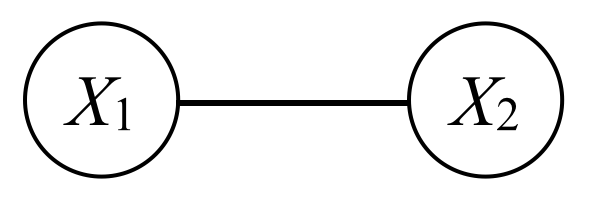
\includegraphics[scale=0.4]{images_sec-graphical-models-2-rv-possibly-dependent} \par}

Again, the line is there between $X_1$ and $X_2$ precisely because to store the associated joint probability table, regardless of which of the different ways we store the tables, we have to use a table that depends on both $X_1$ and $X_2$.

\textbf{Markov Chain}

Next, suppose we have three random variables $X_1$, $X_2$ and $X_3$, where we make an assumption here that the joint probability table has factorization
{\centering$p_{X_1,X_2,X_3}(x_1,x_2,x_3) = p_{X_1}(x_1) p_{X_2|X_1}(x_2|x_1) p_{X_3|X_2}(x_3|x_2). \qquad \qquad$ (3.1) \par}

Note that this factorization is in general not true for three random variables $X_1$, $X_2$ and $X_3$.

To see, this, we can apply the product rule (which is true for any three random variables $X_1$, $X_2$ and $X_3$):
{\centering$p_{X_1,X_2,X_3}(x_1,x_2,x_3) = p_{X_1}(x_1) p_{X_2|X_1}(x_2|x_1) p_{X_3|X_1, X_2}(x_3|x_1, x_2). \qquad \qquad$ (3.2) \par}

To see what the assumption that equation (3.1) holds means, we equate it with the equation from the product rule (3.2) to get

{\renewcommand{\arraystretch}{1.5}
\begin{tabular}{l l}
 & $p_{X_1}(x_1) p_{X_2|X_1}(x_2|x_1) p_{X_3|X_2}(x_3|x_2)$ \\ 
 & $= p_{X_1,X_2,X_3}(x_1,x_2,x_3)$ \\
 & $= p_{X_1}(x_1) p_{X_2|X_1}(x_2|x_1) p_{X_3|X_1, X_2}(x_3|x_1, x_2)$,	 
\end{tabular}}
				
from which we deduce that $p_{X_3|X_1,X_2}(x_3|x_1,x_2)=p_{X_3|X_2}(x_3|x_2)$. This means that given $X_2$, knowing $X_1$ does not tell us anything new about $X_3$:
{\centering$X_1 \perp X_3 \mid X_2.$ \par}
 
So assuming equation (3.1) holds means that we are making an assumption about conditional independence structure!

Next, let's see how to store the distribution when it has factorization given by equation (3.1). We see that it suffices to keep track of three tables $\phi_1$, $\psi_{1, 2}$, and $\psi_{2, 3}$:

{\centering$p_{X_1,X_2,X_3}(x_1,x_2,x_3) = \underbrace{p_{X_1}(x_1)}_{\phi _1(x_1)} \underbrace{p_{X_2|X_1}(x_2|x_1)}_{\psi _{1, 2}(x_1, x_2)} \underbrace{p_{X_3|X_1, X_2}(x_3|x_1, x_2)}_{\psi _{2, 3}(x_2, x_3)}.$ \par}
 
The graph associated with this representation has three circles, one for each of the random variables $X_1$, $X_2$ and $X_3$. We have a table $\psi_{1, 2}$ that depends on $X_1$ and $X_2$ so we draw a line between the circles for $X_1$ and $X_2$. Next we have a table $\psi _{2, 3}$ that depends on $X_2$ and $X_3$ so we draw a line between the circles for $X_2$ and $X_3$. This yields the following:

{\centering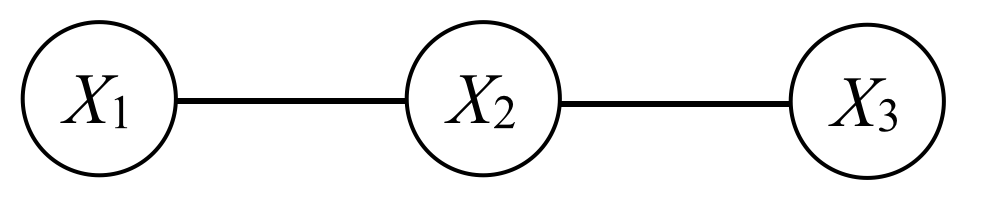
\includegraphics[scale=0.4]{images_sec-graphical-models-3-rv-markov-chain} \par}

This line-shaped graph is called a Markov chain. We will encounter Markov chains more later on. Notationally, when $X_1$, $X_2$ and $X_3$ form a Markov chain, we write $X_1 \leftrightarrow X_2 \leftrightarrow X_3$.

\textbf{The General Case}

We are almost ready to mathematically define what a graphical model is. As we saw from the above examples, each time we had a graph (a picture with circles and possibly lines) along with tables that we store.

For a graph, the circles are formally called nodes or vertices, and the lines are formally called edges. The graph is undirected because the edges do not have directionality associated with them. Furthermore:

Each node corresponds to a random variable

Each edge indicates there being some possible dependence between the two nodes that it connects. Specifically: an edge being present between two nodes $X_i$ and $X_j$ means that the equation for the probability distribution has a factor that depends on both $X_i$ and $X_j$; this factor is stored as table $\psi_{i, j}$.

From these definitions, an important concept emerges: More edges implies that the model can encode more probability distributions but we have to store more tables. (Think about why the second example we presented for two random variables where we don't know whether they're independent or not (and had a factor $\psi_{1, 2}$) can actually encode a distribution in which $X_1$ and $X_2$ are independent!)

Meanwhile, in the graphs that we will consider, we will assume that there are no loops. We do this for simplicity: probabilistic graphical models with loops are beyond the scope of this course.

Note that a graph is specified by saying what the nodes (circles) are, and what the lines (edges) are. To give specific examples:

\begin{itemize}
\item When $X_1$ and $X_2$ were independent, the graph we had consisted of the set of nodes $V=\{ 1, 2\}$ and the set of edges $E=\emptyset$.

\item When $X_1$ and $X_2$ were not known as to whether they are independent or not, the graph we had consisted of the set of nodes $V=\{ 1, 2\}$ and the set of edges $E=\{(1,2)\}$. Note that in general we use $(i,j)$ to mean an edge between nodes $i$ and $j$, where $(i,j)$ and $(j,i)$ mean the same thing, which is why the set of the edges here includes only $(1,2)$and not both $(1,2)$ and $(2,1)$.

\item When we have $X_1 \leftrightarrow X_2 \leftrightarrow X_3$, the set of nodes is $V=\{1,2,3\}$ and the set of edges is $E=\{(1,2),(2,3)\}$.
\end{itemize}

\paragraph{Definition of an undirected pairwise graphical model} (we will just call this a graphical model): An \textit{undirected pairwise graphical model} for random variables $X_1, \dots , X_n$ consists of an undirected graph with vertices $V=\{1, \dots ,n\}$ and edges $E$, and tables $\phi_i$'s and $\psi_{i, j}$'s that have nonnegative entries. The joint probability table of $X_1, \dots , X_n$ is given by

{\centering$p_{X_1, \dots , X_ n}(x_1, \dots , x_ n) =\frac{1}{Z}\prod _{i\in V}\phi _{i}(x_{i})\prod _{(i,j)\in E}\psi _{ij}(x_{i},x_{j}),$ \par}

where $Z$ is the normalization constant that ensures that the probability distribution actually sums to 1 (we'll give a concrete example shortly).

Note that in earlier examples, we didn't always specify that a random variable $X_i$ needed to have a table $\phi_i$. This is not a problem: we can just set $\phi_i(x_i) = 1$ for all values of $x_i$ in this case.

\textbf{Terminology:}

Each table $\phi_i$ depends only on random variable $X_i$ and is called the node potential function or node potential of node $i$.

Each table $\psi_{i, j}$ depends only on random variables $X_i$ and $X_j$ and is called the pairwise potential function or pairwise potential or edge potential of nodes $i$ and $j$.

\paragraph{Important:} We require that the potential tables consist of nonnegative entries \textbf{but each potential table does not have to sum to 1}. The constant $Z$ will ensure that the joint probability table actually sums to 1.


\subsection{Trees}

A tree is a graph for which there are no loops, and we can reach from any node to any other node (moving along edges in the graph). We'll be seeing trees quite a bit so here are some basics of trees.

\textbf{Example:}

{\centering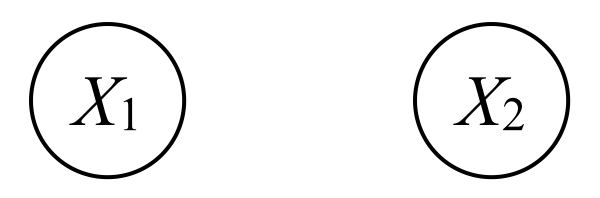
\includegraphics[scale=0.4]{images_sec-graphical-models-2-rv-indep} \par}

This graph is not a tree since there is no path from $X_1$ to $X_2$.

\textbf{Example:}

{\centering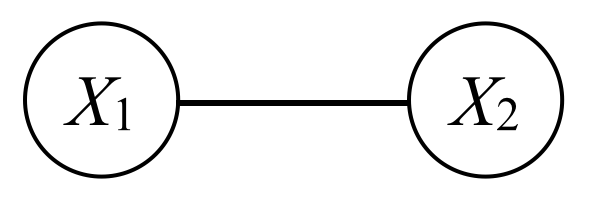
\includegraphics[scale=0.4]{images_sec-graphical-models-2-rv-possibly-dependent} \par}

This graph is a tree since there are no loops and we can reach from any node to any other node.

\textbf{Example:}

{\centering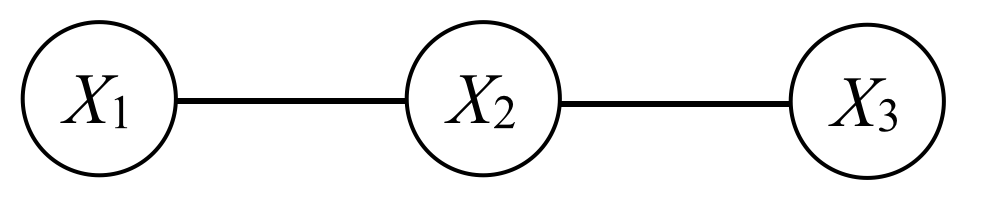
\includegraphics[scale=0.4]{images_sec-graphical-models-3-rv-markov-chain} \par}

This graph is a tree since there are no loops and we can reach from any node to any other node.

\paragraph{Theorem:} For any graph that has $n$ nodes, if the graph is a tree, then it will always have exactly $n-1$ edges.

\paragraph{Proof:} We use induction.

Base case $n=1$: There is only 1 node so there are no edges, so the claim clearly holds.

Inductive step: Suppose the claim holds for every tree of size (i.e., number of nodes) up to $k$. Thus, every tree of size $k$ nodes has $k-1$ edges. Now consider a tree $T$ with $k+1$ nodes. Take a leaf node $v$ from $T$ and note that the tree $T$ with $v$ removed is a tree $T?$ of size $k$, which by the inductive hypothesis has $k-1$ edges. Since $v$ is a leaf node though, it has exactly 1 neighbor, which means that the tree $T$ has 1 more edge than the tree $T?$, i.e., $T$ has $k$ edges. This finishes the inductive step. $\square$

\subsection{Practice Problem: Computing the Normalization Constant }

It turns out that once we know the potential functions, the normalization constant $Z$ becomes fixed since the distribution needs to sum to 1. Let's show this for a simple case. Consider a two node graphical model with an edge between the two nodes corresponding to

{\centering$p_{X_{1},X_{2}}(x_{1},x_{2})=\frac{1}{Z}\phi _{1}(x_{1})\phi _{2}(x_{2})\psi _{12}(x_{1},x_{2}).$ \par}
 
Suppose that we are given what the potential functions are. Show what $Z$ is equal to as a function of $\phi_{1}$, $\phi_{2}$, and $\psi_{12}$.

Hint: Sum both sides over all values of $x_1$ and all values of $x_2$. What is $\sum _{x_{1}}\sum _{x_{2}}p_{X_{1},X_{2}}(x_{1},x_{2})$ equal to?

Because knowing the potentials fixes what the value of $Z$ is, often times we'll omit writing $Z$ and instead write

{\centering$p_{\underline{X}}(\underline{x})\propto \prod _{i\in V}\phi _{i}(x_{i})\prod _{(i,j)\in E}\psi _{ij}(x_{i},x_{j}),$ \par}
 
where ``$\propto$'' means ``proportional to''.

\paragraph{Solution:} We have

{\renewcommand{\arraystretch}{1.5}
\begin{tabular}{l l l}
1 & $=$ & $\sum _{x_{1}}\sum _{x_{2}}p_{X_{1},X_{2}}(x_{1},x_{2})$ \\
  & $=$ & $\sum _{x_{1}}\sum _{x_{2}}\frac{1}{Z}\phi _{1}(x_{1})\phi _{2}(x_{2})\psi _{12}(x_{1},x_{2})$ \\
  & $=$ & $\frac{1}{Z}\sum _{x_{1}}\sum _{x_{2}}\phi _{1}(x_{1})\phi _{2}(x_{2})\psi _{12}(x_{1},x_{2}),$ 
\end{tabular}}

so

{\centering$Z=\sum _{x_{1}}\sum _{x_{2}}\phi _{1}(x_{1})\phi _{2}(x_{2})\psi _{12}(x_{1},x_{2}).$ \par}
 
In general for a graphical model with graph $G=(V,E)$ and factorization

{\centering$p_{X_{1},\dots ,X_{n}}(x_{1},\dots ,x_{n})=\frac{1}{Z}\prod _{i\in V}\phi _{i}(x_{i})\prod _{(i,j)\in E}\psi _{ij}(x_{i},x_{j}),$ \par}
 
using the same reasoning as above,

{\centering$Z=\sum _{x_{1}}\cdots \sum _{x_{n}}\prod _{i\in V}\phi _{i}(x_{i})\prod _{(i,j)\in E}\psi _{ij}(x_{i},x_{j}).$ \par}
 



\end{document}
